 
  \documentclass[final]{beamer} % beamer 3.10: do NOT use option hyperref={pdfpagelabels=false} !

  %\documentclass[final,hyperref={pdfpagelabels=false}]{beamer} % beamer 3.07: get rid of beamer warnings
  \mode<presentation> {  %% check http://www-i6.informatik.rwth-aachen.de/~dreuw/latexbeamerposter.php for examples
    \usetheme{Berlin}    %% you should define your own theme e.g. for big headlines using your own logos 
  }
\setbeamercolor{block body}{bg=white, fg=black}
\setbeamerfont{block title}{size=\Large}
\usepackage{lmodern}

  \usepackage[english]{babel}
  \usepackage[latin1]{inputenc}
  \usepackage{amsmath,amsthm, amssymb, latexsym}
  \usepackage{float}
  \usepackage{booktabs}
\usepackage{mathptmx}
\usepackage{color}
\usepackage{pgfplots}
\usepackage{anyfontsize}
  %\usepackage{times}\usefonttheme{professionalfonts}  % times is obsolete
  \usefonttheme[onlymath]{serif}
  \boldmath
  \usepackage[orientation=portrait,size=a0,scale=1.10, debug]{beamerposter}                       % e.g. for DIN-A0 poster
  %\usepackage[orientation=portrait,size=a1,scale=1.4,grid,debug]{beamerposter}                  % e.g. for DIN-A1 poster, with optional grid and debug output
  %\usepackage[size=custom,width=200,height=120,scale=2,debug]{beamerposter}                     % e.g. for custom size poster
  %\usepackage[orientation=portrait,size=a0,scale=1.0,printer=rwth-glossy-uv.df]{beamerposter}   % e.g. for DIN-A0 poster with rwth-glossy-uv printer check
  % ...
\definecolor{OliveGreen}{HTML}{eeeeee}

\begin{document}

  \begin{frame}
    \begin{center}

      \textcolor{black}{
      \textbf{\fontsize{110}{200}{\selectfont Panthera: Caching and Cache-based Scheduling}}
      \vspace{0.5em}
      \textbf{\fontsize{110}{200}{\selectfont in Distributed Computing Systems}}}
    \end{center}
    
    \begin{columns}[t]
     \begin{column}{0.32\textwidth}
      \begin{block}{Introduction}
      \textbf{Distributed computing} has seen tremendous growth in the past few years.
Essentially, it allows computational algorithms to execute over a network (i.e.
\textit{\textbf{cluster}}) of computers. This project is focused on the \textbf{\textit{Hadoop}} distributed
computing system, which has found extensive use throughout academia and
industry. For example, major software companies such as Yahoo, Microsoft, Facebook, Cloudera, etc. all utilize Hadoop heavily. Hadoop provides a mechanism (called a \textit{\textbf{distributed filesystem}}) that 
allows each computer (i.e. \textit{\textbf{node}}) in a cluster to access the same set of files.
However, it fails to utilize local Random Access Memory (RAM) resources to reduce the waiting
time (i.e. \textbf{\textit{latency}}) associated with obtaining these files. \textbf{This project develops and tests scheduling and caching mechanisms to reduce latency in Hadoop, thereby greatly increasing Hadoop's efficiency and applicability in fields ranging from bioinformatics to artificial intelligence.}

	%%%%%%%%%%%%%%%%%%%%%%%%%%%%%%%5
      %\textbf{Distributed computing} has seen tremendous growth in the past few years. Essentially, it allows 
      %In particular, Hadoop is an open source distributed computing system
      %used throughout academia and industry. For example, Yahoo, Facebook, Microsoft, etc.
      %contribute to its development. Hadoop Essentially, it allows computational algorithms to execute across a \textit{cluster}
      %of computers. In order to facilitate this, distributed computational systems must make files accessible all all the \textit{nodes} of a computer cluster. 
      %\textbf{Distributed computing} has seen tremendous growth in the past few years. 
      %Essentially, \textbf{it allows computational algorithms to execute across multiple
      %computers (i.e. \textit{nodes})}. Most distributed systems must make files accessible over 	networks of computers. \textbf{\textit{Hadoop}} is an open source and heavily used distributed computing sytem. It has found extensive applications in academia and industry. For example, Yahoo, Facebook, Microsoft, etc. are all heavily involved with Hadoop development. But, Hadoop does not effectively utilize Random Access Memory (RAM) and local storage to better performance. \textbf{This project develops and tests scheduling and caching mechanisms to reduce waiting time (i.e. latency) in Hadoop, thereby greatly increasing Hadoop's efficiency and applicability in fields ranging from bioinformatics to artificial intelligence.}
      %%%%%%%%%%%%%%%%%%%%%%%%%%%55
      
      %\textbf{Distributed computing} has seen tremendous growth in the past few years. Essentially, \textbf{it allows computational algorithms to execute across multiple computers (i.e. \textit{nodes})}. Most distributed computing systems must make files accessible over networks of computers so that a given algorithm being executed has access to its input data. However, obtaining these files has an associated waiting time, known as $\textit{\textbf{latency}}$. \textbf{This project aims to reduce latency within
      %distributed computing systems to reduce the time algorithms take to run}.
      
      %\textbf{This 
      %project aims to reduce the waiting time (known as \textit{latency}) associated
      %with obtaining files within distributed computing systems}.
      %\end{block}
      %\begin{block}{Introduction}
      %\textbf{\textit{Hadoop}} is an open source and heavily used distributed computing sytem. It has found extensive applications in academia and industry. For example, Yahoo, Facebook, Microsoft, etc. are all heavily involved with Hadoop development. But, Hadoop does not effectively utilize Random Access Memory (RAM) and local storage to better performance. \textbf{This project develops and tests scheduling and caching mechanisms to reduce latency in Hadoop, thereby greatly increasing Hadoop's efficiency and applicability in fields ranging from bioinformatics to artificial intelligence.}
      \end{block}

	\begin{block}{Past Research}
	\begin{itemize}
		\item Several sources (e.g. T. White) have identified latency as a core problem in Hadoop's architecture. However, cache-based latency reduction has been unexplored.
		\item Schedulers have been developed for Hadoop (by M. Zaharia, Y. He, etc.), though none have utilized file storage information.
		\item A wide range of algorithms for operating system-level scheduling exist, but Hadoop's architecture requires a fairly ad-hoc approach.
	\end{itemize}
	\end{block}
	
	\begin{block}{Caching}
	There is significant waiting time/latency associated with retrieving files from distributed filesystems. \textbf{Caches} are used to store
	some files in local RAM so that they can be accessed much more quickly. Panthera implements a cache and a cache-based scheduler for Hadoop.
	\end{block}
	
    \begin{block}{Problem}
	\begin{itemize}
	 \item \textbf{Develop a caching layer} for the Hadoop Distributed File System that can cache \textbf{both data and metadata}.
	 \item The solution should be a \textbf{``drop-in'' addition}, allowing for easy adoption and integration into existing systems.
	 \item The layer \textbf{should reduce file access latency} significantly in comparison to \textbf{the control group: a standard Hadoop installation}.
	 \item \textbf{Develop a scheduler} for the Hadoop which \textbf{schedules jobs based on what is available in the cache}. In addition, it should be be able to \textbf{prefetch files that could be needed in the future}.
	\end{itemize}

      \end{block}

      \begin{block}{Hypothesis}
       The cache layer designed (called \textbf{Panthera}) will have lower file
       access latency when compared to a standard Hadoop installation. Additionally, it
       will be possible to design \textbf{Panthera} such that the Hadoop source code
       remains unaffected. It will also be feasible to create a cache-based 
       scheduler for Hadoop.
      \end{block}
	  
		\begin{block}{Data vs Metadata}
			\begin{itemize}
				\item \textbf{Data} within the Hadoop file system \textbf{consists of the actual contents of a file.}
				\item \textbf{Metadata is information \textit{about} files and directories}, e.g. time a file was created, the list of files in a directory, etc.
				\item \textbf{Panthera performs both metadata
			and data caching; both have significantly different technical implications
			and challenges.}
			\end{itemize}
		\end{block}
	
		\begin{block}{Current Hadoop File System Architecture}
			\centerline{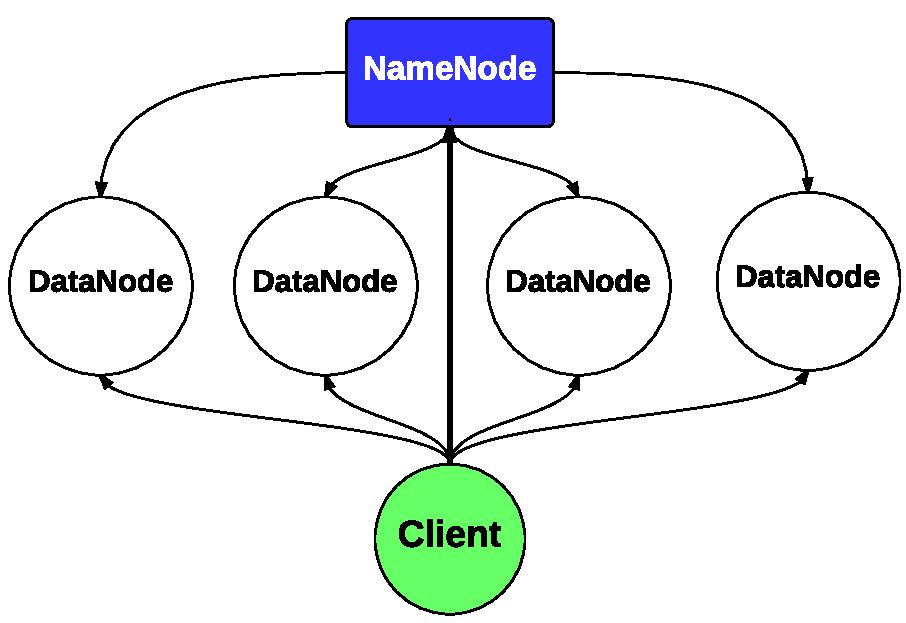
\includegraphics[scale=1.4]{assets/v2/vanilla_hadoop_arch.pdf}}
		\end{block}
	
		\begin{block}{Latency Types - Theory}
		%discuss the types of latency and make the comparison
		%between hard disk latency and regular lateny
		In the Hadoop File System Architecture, there are several types of latencies involved (listed from highest to lowest magnitude):
		\begin{itemize}
		\item \textbf{Network latency}
		\item \textbf{Hard drive latency}
		\item \textbf{Memory latency: } Reading from RAM memory has an extremely small
		waiting time associated with it ($<$ 1/100th that of the hard drive). \textbf{Panthera converts hard drive and network latency to memory latency, and thus greatly reduces file access time.}
		\end{itemize}
	  	\end{block}
	  

     \end{column}
     %##########################################################################################################

    \begin{column}{0.32\textwidth}
		\begin{block}{Panthera Architecture}
		\vspace{0.5em}
		\centerline{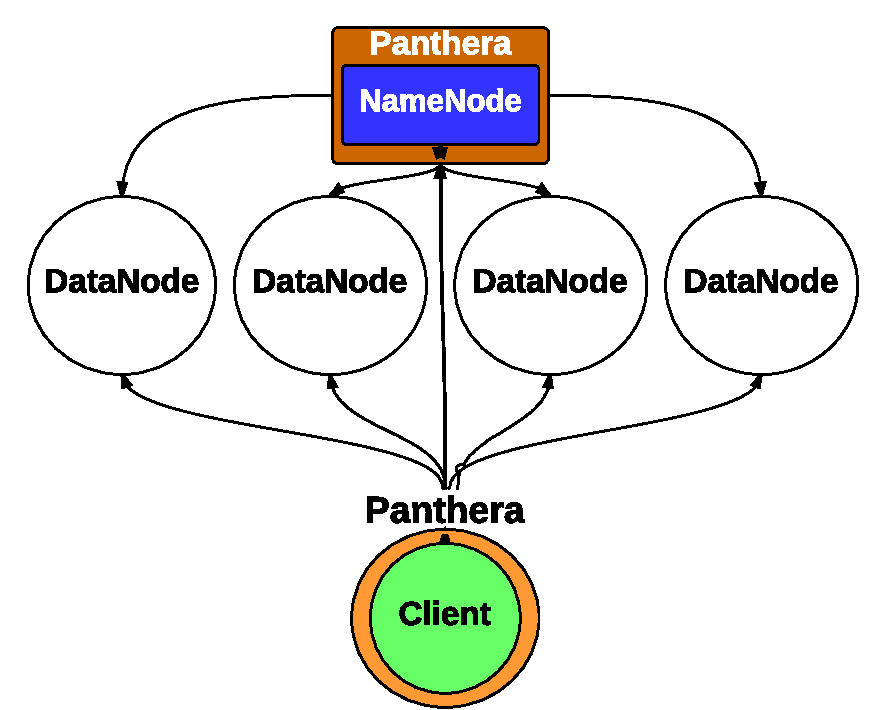
\includegraphics[scale=1.4]{assets/v2/panthera_hadoop_arch.pdf}}	  
	  \end{block}   	  
		%\begin{block}{Panthera Metadata Architecture}
	 		%\centerline{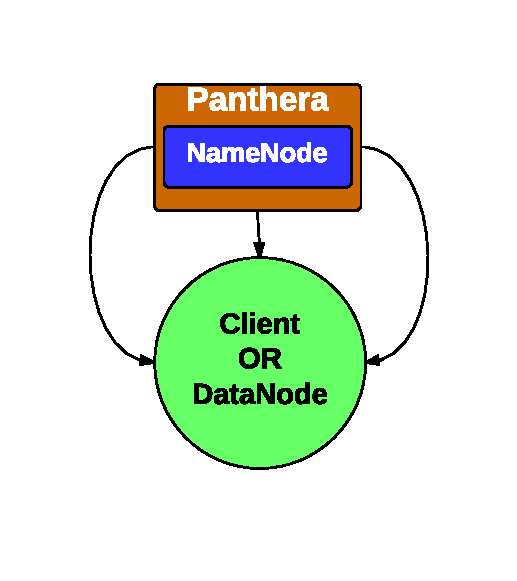
\includegraphics[scale=1.2]{assets/panthera_metadata_large.pdf}}
      	%\end{block}


      
      %\begin{block}{Panthera Data Architecture}
      %\centerline{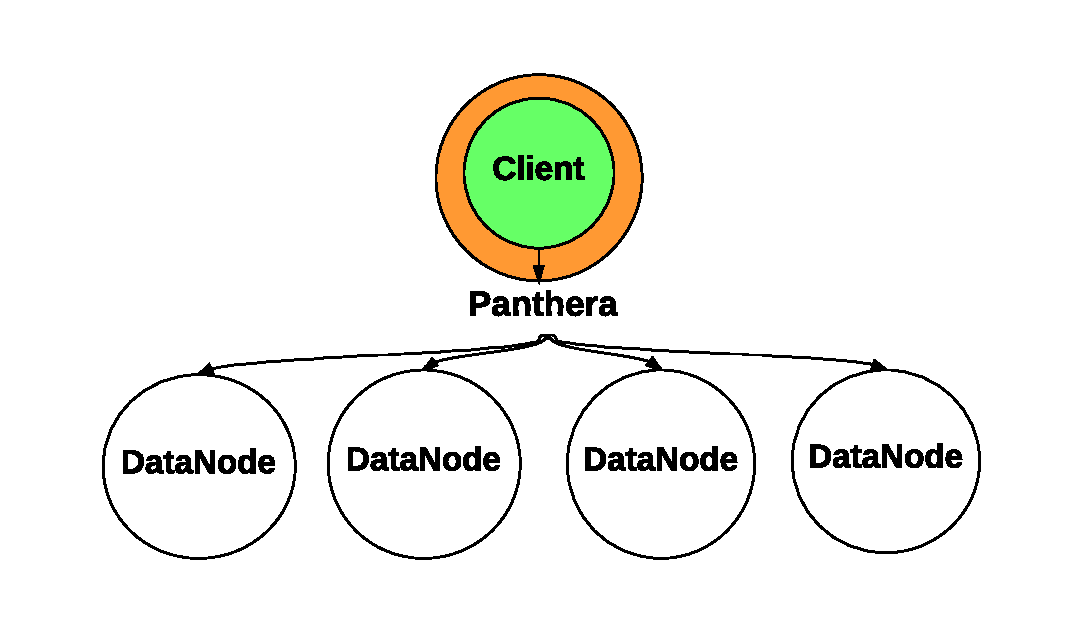
\includegraphics[scale=1.2]{assets/panthera_data_architecture.pdf}}
     %\end{block}

	\begin{block}{Panthera - Implementation}
	\begin{itemize}
		\item \textbf{Panthera is implemented in Google's Go programming language} which has excellent concurrency primitives and memory management, making it perfect for software that must run reliably with hundreds of clients.
	\end{itemize}
	\end{block}
	
	\begin{block}{Latency Testing Methodology}
	Client and server are on separate machines for latency testing.
	\begin{itemize}
		\item \textbf{Metadata}: Repeatedly request directory listing for a directory with 100 files in it.
		\item \textbf{Data}: Repeatedly request file contents for a 64MB file (64MB = 1 block in Hadoop).
	\end{itemize}

	\end{block}
		\begin{block}{Latency Results}
		\vspace{1em}
		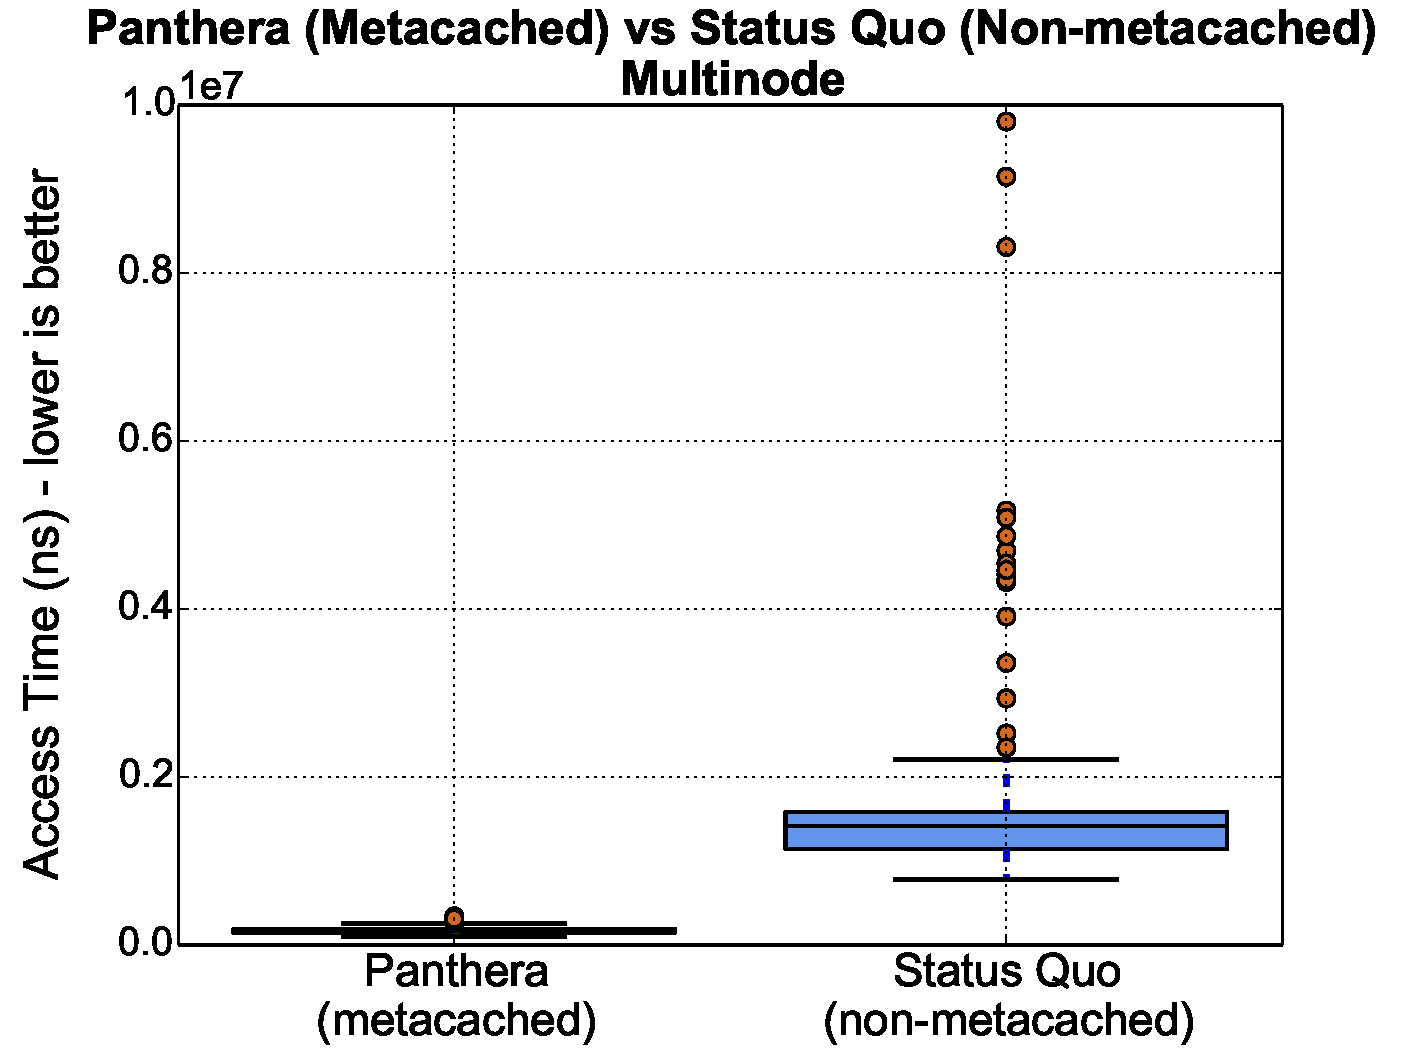
\includegraphics[scale=1]{assets/v2/multinode_meta_box_plot.pdf}
		\vspace{1.5em}
		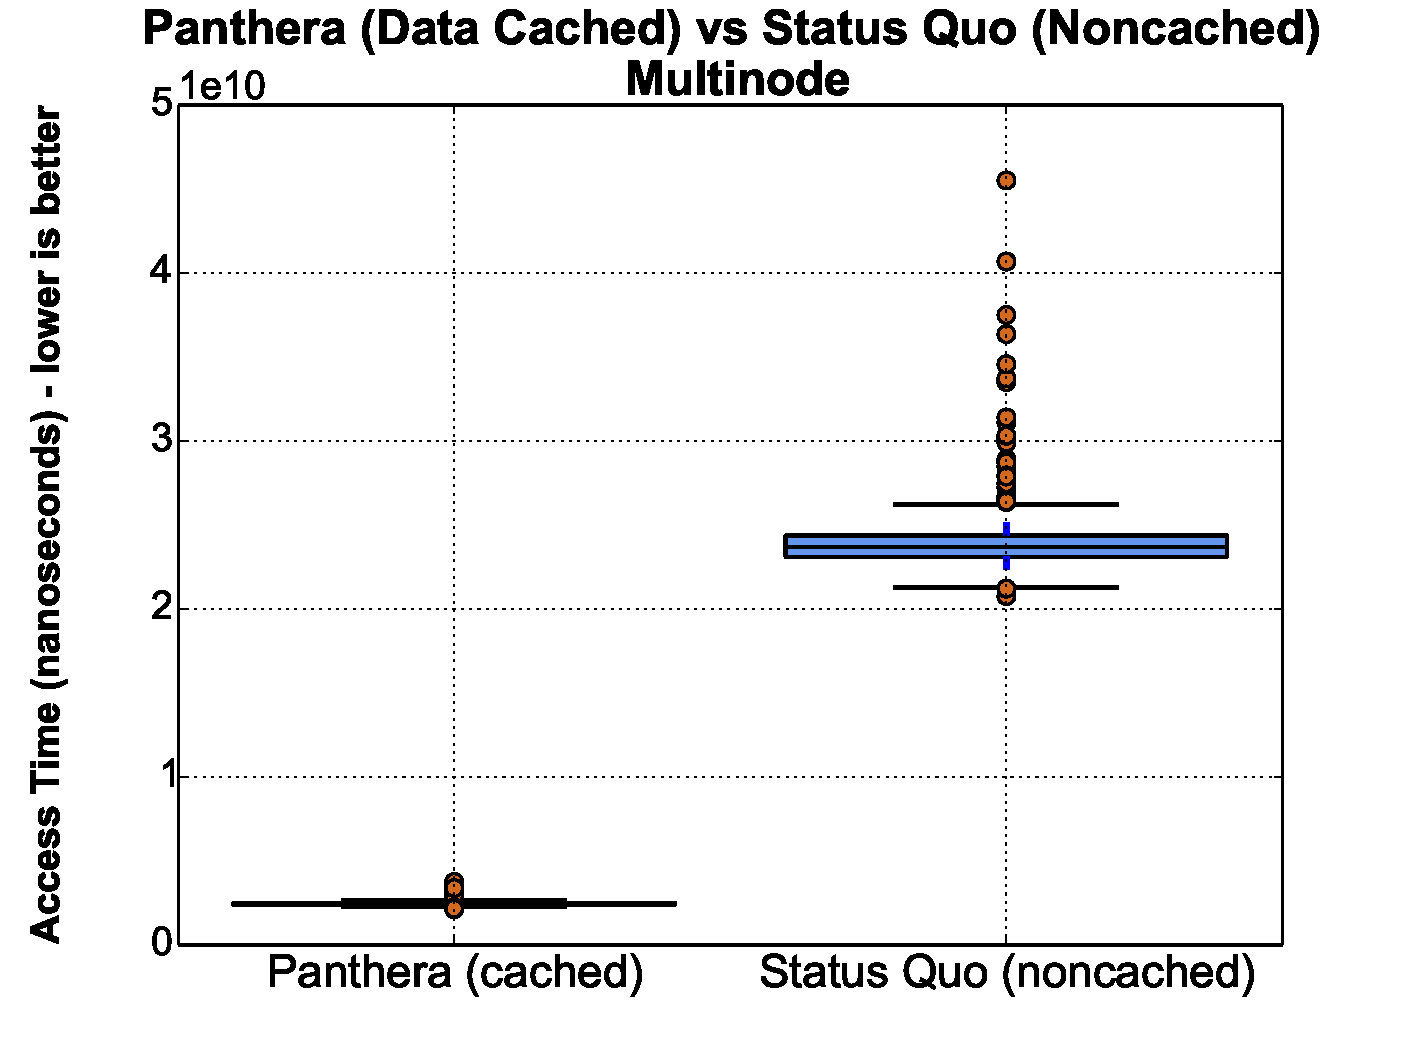
\includegraphics[scale=0.98]{assets/v2/getter_boxplot.pdf}
		%\vspace{1em}
		%\includegraphics[scale=0.98]{assets/v2}
	\end{block}
	
	\begin{block}{Procedure Testing Methodology}
	Panthera was also tested with running times of algorithms executing on Hadoop (as opposed to only downloading data or metadata). The input sample to both algorithms tested was a repeated copy of "The 
	Adventures of Sherlock Holmes" (192 MB). Algorithms tested: 
	\begin{itemize}
	\item \textbf{WordCount}: A classic distributed algorithm that counts occurrences of all words in a given text.
	\item \textbf{ReferenceCount}: Counts occurrences of words in a given text, but 
	only considers the words that are in a given reference file.
	\end{itemize}
		\vspace{1.5em}
		\centerline{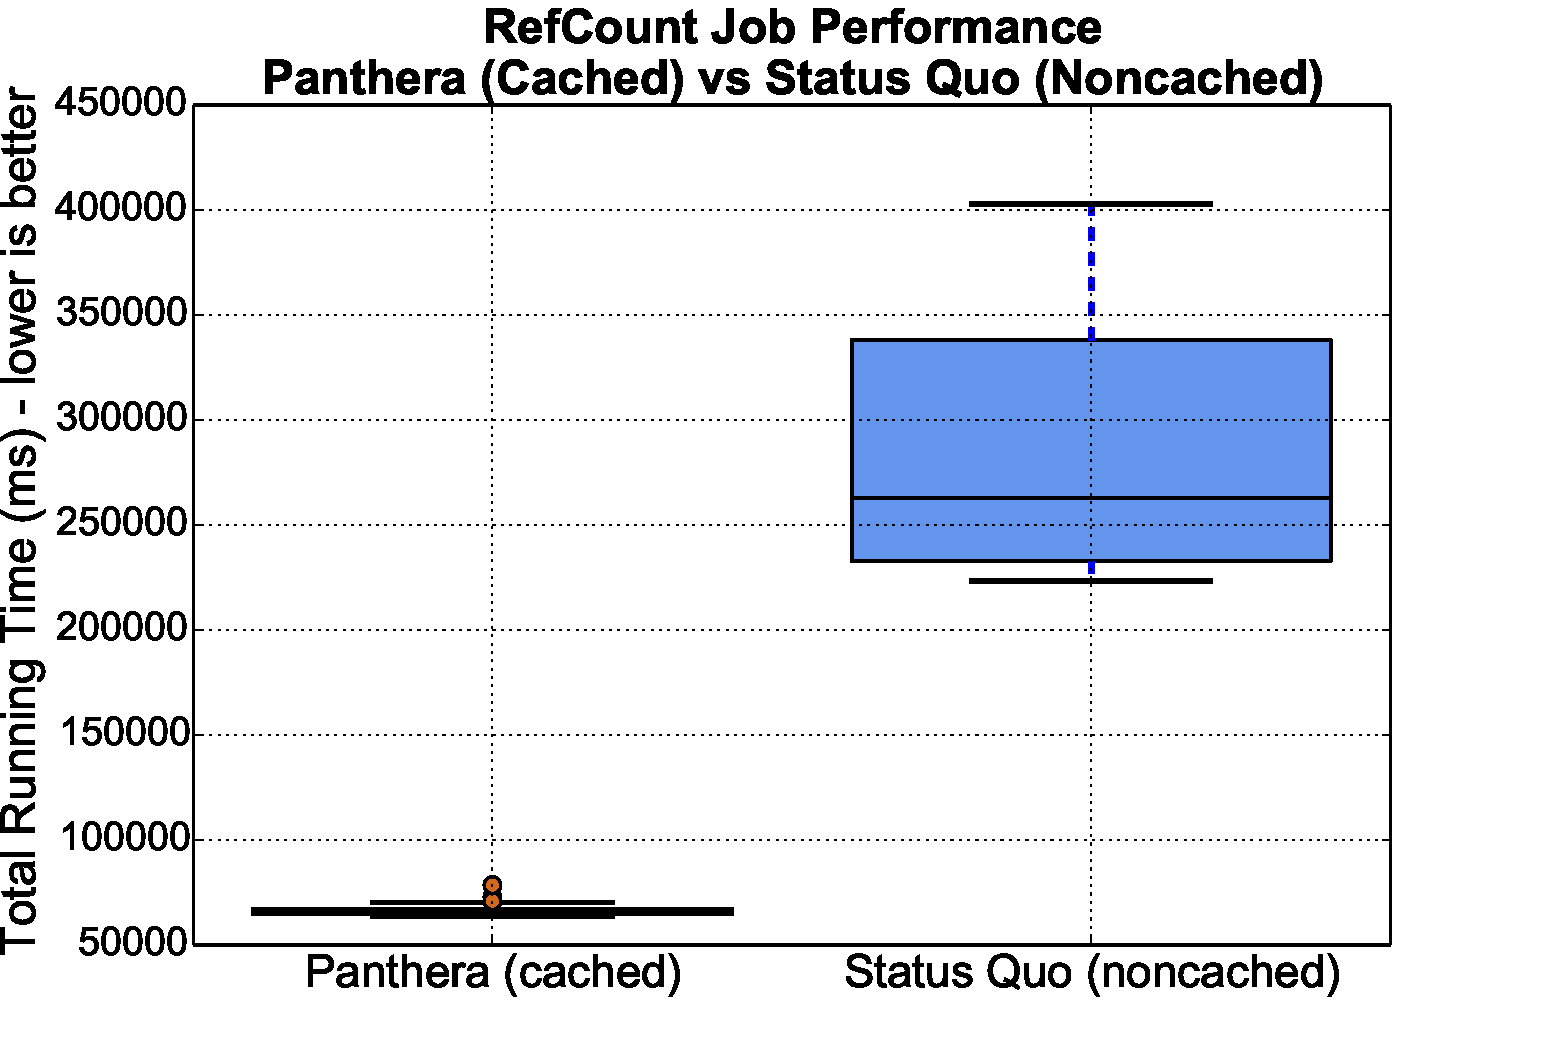
\includegraphics[scale=1]{assets/v2/refgetter_boxplot.pdf}}
		\end{block}


	  
      \end{column}
      %##########################################################
            \begin{column}{0.32\textwidth}
      		\begin{block}{Panthera Scheduling Algorithm Theory}
		\begin{itemize}
			\item \textbf{Problem}: Given $\mathbf{J} = J_1, J_2, ... ,J_k$ jobs to be run
			on a Hadoop cluster with caches $\mathbf{C} = C_1, C_2, ..., C_n$, what ordering will best take advantage of the caches?
			\item \textbf{Panthera job score}: Each $J_i$ accesses a set of blocks $F_i$
			and each $C_i$ holds a set of blocks $B_i$.
			Every $J_i$ is assigned a job score $x_i$:
			\begin{equation}
				x_i = \displaystyle{\frac{\left\vert{F_i \cap B_t}\right\vert}{ \left\vert{B_t}\right\vert}} \; \textrm{where} \;
				B_t = \bigcup_{j = 1}^{n} B_j
			\end{equation}
			\item \textbf{Panthera scheduling algorithm}:
			Sort $\mathbf{J}$ in descending order with respect to the $x_i$ associated
			with each $J_i$. While $J_i$ is running, Panthera may prefetch data for $J_{i+1}$ to further reduce latency.
		\end{itemize}
		\end{block}
	
	
	
    \begin{block}{Statistics}
	\begin{table}
	\setlength{\tabcolsep}{25pt}
	\centering
	\begin{tabular}{lc}
		\toprule
		\textbf{Type} & \textbf{Mean time improvement} \\
		\midrule
		Metadata   & 8.13x \\
		Data       & 8.63x \\
		Word count & 1.25x \\
		Ref. count & 3.31x \\
	\bottomrule
	\end{tabular}
	\caption{Improvement with Panthera in the total amount of time required to execute algorithms/requirements (compared with status quo). \textbf{An improvement of "3x" implies that the mean time was 3 times lower with Panthera compared to the status quo.}}
	\end{table}
 	
 	\vspace{1em}
	\begin{table}
	\setlength{\tabcolsep}{25pt}
	\centering
	\begin{tabular}{lc}
		\toprule
		\textbf{Type} & \textbf{Standard deviation contraction} \\
		\midrule
		Metadata   & 27.38x \\
		Data       & 11.14x \\
		Word count &  \phantom01.02x \\
		Ref. count & 22.91x \\
	\bottomrule
	\end{tabular}
	\caption{Reduction obtained with Panthera in the standard deviation of running times, i.e. a \textbf{contraction of 9x implies that the standard deviation was reduced
	by a factor of 9 with Panthera compared to the status quo.}}
	\end{table}

    \end{block}
    
    	\begin{block}{Conclusion}
    	The results validate the hypothesis presented.
    	\begin{itemize}
    		\item Panthera was successfully developed as a "drop-in" solution
    		\item It was able to reduce latency in comparison to a standard Hadoop installation. 
    		\item A scheduler was also implemented which uses cache information to schedule
    		Hadoop jobs.
    		\item Metadata latency was \textbf{decreased by a factor of 8.13}
    		\item Data latency was \textbf{decreased by a factor of 8.63}
    		\item The running of time of WordCount (an algorithm with very few file accesses) was \textbf{improved by 25.1\%} with the code left unmodified.
		\item The running time of RefCount was \textbf{improved by a factor of 3.31} with its code also unmodified.
    	\end{itemize}
	 
    Thus, Panthera can significantly improve existing distributed systems
    without any code modifications and also enable developers to 
    implement algorithms that were previously impractical (such as RefCount).
	
	\end{block}
	
	\begin{block}{Applications}
	Panthera can be applied in a vast range of disciplines since the Hadoop
	distributed system is in widespread use. A few examples follow: 
	\begin{itemize}
		\item \textbf{Machine Learning}
			\begin{itemize}
			\item Panthera was tested with Apache Mahout, which is a library of machine learning algorithms for Hadoop
			\end{itemize}
			
		\item \textbf{Bioinformatics}
			\begin{itemize}
				\item BioDoop: a bioinformatics framework for Hadoop.
				\item Distributed sequence alignment
			\end{itemize}
			
		\item \textbf{Predictive Analytics}	
			\begin{itemize}
				\item Hadoop is heavily used for predictive analytics. Panthera can
				be used to reduce the running time of queries and schedule queries
				for maximal efficiency, reducing total turnaround time.
			\end{itemize}
		\item \textbf{Image Processing}
		\item \textbf{Numerical/Scientific Computing}
		\begin{itemize}
			\item Apache Hama is a matrix computational package for Hadoop. Applications using it can be made more efficient without any modifications to their codebases due to Panthera's ``drop-in'' nature,.
			\end{itemize}
			
	\end{itemize}
	Due to the drastic decreases in latency and running times that Panthera provides
	(in addition to allowing the implementation of previously impractical algorithms), \textbf{Panthera can truly transform computational work across many
	fields of study.}
	\end{block}
	
	\begin{block}{Future Work}
	\begin{itemize}
		\item \textbf{All code developed during this project will be open sourced to further development in distributed computing.}
		\item Expose an API to allow external caching requests (almost complete)
		\item Currently working on testing a \textbf{bioinformatics toolkit with Panthera}; initial results are very promising and show significant reduction in total running time.
		\item Implement \textbf{predictive prefetching} algorithms on Panthera
		\item Consider the effects of different cache replacement algorithms
		
	\end{itemize}
	\end{block}
      \end{column}
    \end{columns}
  \end{frame}
    
  \end{document}